\subsection{Mediator}


Nesse padrão, um objeto chamado de Mediator age como intermediário 
entre um grupo de objetos, fazendo com que qualquer interação entre 
eles seja encapsulada em um único objeto. O Mediator conhece todos 
esses objetos, enquanto cada objeto conhece apenas o 
Mediator. Dessa forma, os objetos que precisam comunicar-se são 
mais independentes, simplificando a reutilização dos 
mesmos e concentrando as dependências entre eles 
em um só lugar. 

A estrutura do padrão é apresentada na figura \ref{mediator_struct}. 
Uma interface Mediator define as operações que um tipo de 
objeto Mediator deve possuir. ConcreteMediator representa 
uma classe que implementa essas operações. Um Colleague 
é um objeto conhecido pelo Mediator e cada ConcreteColleague 
pode ser tanto um objeto que possui operações refletidas 
em outros objetos quanto ser um dos objetos alterados 
indiretamente.


\begin{figure}[htb]
	\caption{\label{mediator_struct}Estrutura do Mediator}
	\begin{center}
	    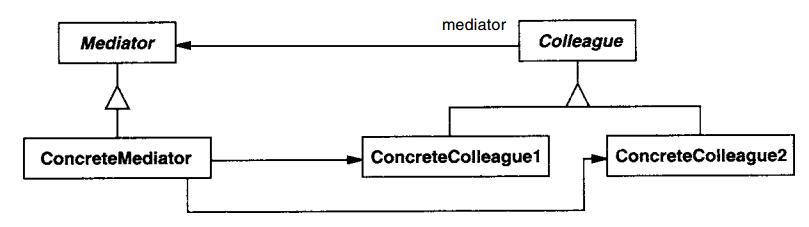
\includegraphics[scale=0.5]{5_padroes-contexto-funcional/5.3_comportamentais/5.3.05_mediator/diagram.png}
	\end{center}
\end{figure}



\subsubsection*{Exemplo Orientado a Objetos}





\begin{lstlisting}[caption={Mediator Orientação a Objetos},label=oomediator]

trait DialogDirector {
    
    def ShowDialog() {
        // Operação que exibe o Dialog
    }

    def CreateWidgets() : Unit
    def WidgetChanged(widget : Widget) : Unit
}

class FontDialogDirector extends DialogDirector {
    
    val list : ListBox
    val field : EntryField
    
    def CreateWidgets() {
        this.list = new ListBox(this)
        this.field = new EntryField(this)
    }

    def WidgetChanged(widget : Widget) {
        this.field.SetText(
            this.list.GetSelection()
        )
    }

}

abstract class Widget(val director : DialogDirector){

    def Changed() : Unit = this.director.WidgetChanged(this)

}

class EntryField(director : DialogDirector) extends Widget(director) {
    var text : String

    def SetText(text : String) {
        this.text = text
    }
}

class ListBox(director : DialogDirector) extends Widget(director){
    var selection : String

    def GetSelection() : String = selection

    def SetSelection(selection : String) {
        this.selection = selection
        Changed()
    }
}
    
\end{lstlisting}

\subsubsection*{Contexto Funcional}

Para implementar esse padrão, é necessário tratar o objeto 
Mediator como uma função ou um conjunto de funções (uma para 
cada operação que o objeto Mediator possuiria) que recebe 
como parâmetro o valor do Colleague que realiza a operação 
e todos os Colleagues que seriam alterados por essa 
operação.

Caso o processo de armazenar os Colleague seja trabalhoso, 
é possível encapuslar a coleção dos Colleagues em uma 
closure. Uma função deve receber a coleção e retornar 
outra função que recebe os parâmetros necessários (por 
exemplo, uma função ou valor que indique qual dos Colleagues 
é o causador da operação) e realiza de fato a operação 
nos colleagues. Enretanto, caso a lista de Colleagues 
seja alterada pela própria operação do Mediator ou por 
alguma outra modificação durante a aplicação, é necessário 
chamar a função geradora novamente para que a closure 
envolvida pela função do Mediator não fique desatualizada.

\begin{lstlisting}[caption={Mediator Funcional},label=fpmediator]
    
object FontDialogDirector {

	import EntryField._
	import ListBox._
	
	def ChangeWidget(
		listBox : ListBox, 
		selection : String, 
		entryField : EntryField) 
	: (ListBox, EntryField) =
		(SetSelection(listBox, selection), SetText(entryField, selection))
	
}
	
object EntryField {
	
	case class EntryField(val text : String)
	
	def SetText(entryField : EntryField, text : String) = 
		entryField.copy(text)
	def GetText(entryField : EntryField) = entryField.text
}
	
object ListBox {
	
	case class ListBox(val selection : String)
		
	def SetSelection(listBox : ListBox, selection : String) = 
		listBox.copy(selection=selection)
	def GetSelection(listBox : ListBox) = listBox.selection
}
	
    
\end{lstlisting}